% !TeX encoding = UTF-8
% !TeX root = master.tex
% !TeX spellcheck = en_US

\documentclass[17pt, a1paper, portrait, margin=0mm, innermargin=15mm, blockverticalspace=15mm, colspace=15mm, subcolspace=8mm]{tikzposter}

%---------------------------------------------------------------------------------------------------
% tikzposter
%---------------------------------------------------------------------------------------------------

\tikzposterlatexaffectionproofoff

\usetheme{Envelope} 										% Default, Rays, Basic, Simple, Envelope, Wave, Board, Autumn, Desert
\usetitlestyle[titletoblockverticalspace=1.0cm]{Envelope}	% Default, Basic, Empty, Filled, Envelope, Wave, VerticalShading
\useblockstyle{Envelope}									% Default, Basic, Minimal, Envelope, Corner, Slide, TornOut
\usenotestyle{Sticky}										% Default, VerticalShading, Corner, Sticky
\usecolorstyle[colorPalette=BlueGrayOrange]{Spain}			% Default, BlueGrayOrange, GreenGrayViolet, PurpleGrayBlue, BrownBlueOrange | Default, Australia, Britain, Sweden, Spain, Russia, Denmark, Germany
\usebackgroundstyle{Rays}									% Default, VerticalGradation, Rays, BottomVerticalGradation, Empty

\settitle{
	\centering
	\tikz[remember picture,overlay]\node[scale=0.9,anchor=west,xshift=-0.47\linewidth,yshift=5.9cm,inner sep=0pt] {
\includegraphics[width=6cm]{logos/inesc-tec}};
	\tikz[remember picture,overlay]\node[scale=0.99,anchor=west,xshift=-0.47\linewidth,yshift=1.0cm,inner sep=0pt] {
\includegraphics[width=7cm]{logos/feup-white}};
	\begin{minipage}[t]{0.85\linewidth}
		\vbox{
			\@titlegraphic \\[\TP@titlegraphictotitledistance]
			\centering
			\color{titlefgcolor} {\bfseries \huge \scshape \@title \par}
			\vspace*{2em}
			{\huge \@author \par} \vspace*{1em} {\LARGE \@institute}
		}
	\end{minipage}
}



%---------------------------------------------------------------------------------------------------
% Packages
%---------------------------------------------------------------------------------------------------

\usepackage{mathpazo}
\usepackage[utf8]{inputenc}
\usepackage[T1]{fontenc}
\usepackage[english]{babel}
\selectlanguage{english}
\usepackage{graphicx}
\usepackage{grffile}
\graphicspath{{figures/}}
\usepackage{float}
\usepackage{booktabs}
\usepackage{tabu}
\usepackage{rotating}
\usepackage{array}
\usepackage{multirow}
\usepackage{multicol}
\usepackage{url}
\usepackage[hidelinks]{hyperref}
\usepackage{hypcap}
\usepackage[capitalise,noabbrev,nameinlink]{cleveref}
\usepackage[nonumberlist,acronym,nomain,nowarn]{glossaries}
\usepackage[gen]{eurosym}
\usepackage{setspace}
\usepackage[center,figurename=Fig.]{caption}
\captionsetup{font={small,stretch=1.0}}
\glsdisablehyper
\makeglossaries

\makeatletter
\g@addto@macro{\UrlBreaks}{\UrlOrds}
\makeatother

%\overfullrule=3mm

%\newacronym{latex-label}{acronym}{acronym description}



%---------------------------------------------------------------------------------------------------
% Top matter
%---------------------------------------------------------------------------------------------------

\title{\parbox{\linewidth}{\centering Recognition of Banknotes in Multiple Perspectives Using\\Selective Feature Matching and Shape Analysis}}
\author{Carlos M. Costa, Germano Veiga, Armando Sousa\texorpdfstring{\\{\LARGE \ttfamily carlos.m.costa@inesctec.pt, germano.veiga@inesctec.pt, asousa@fe.up.pt}}{}}
\institute{INESC TEC and Faculty of Engineering, University of Porto, Portugal}
%\titlegraphic{
\includegraphics[width=5cm]{logos/inesc-tec}}
\date{May 4, 2016\\{IEEE International Conference on Autonomous Robot Systems and Competitions}}


\begin{document}

\maketitle


%---------------------------------------------------------------------------------------------------
% Sections
%---------------------------------------------------------------------------------------------------

\begin{columns}
	\column{0.5}
	\block{Introduction}{
	\section*{Context}
	\begin{itemize}
		\item Most of commercial transactions are still done using physical currencies
		\item Most currencies banknotes were not designed to be usable by visually impaired people
		\item Detection of counterfeit banknotes can improve the reliability of ATMs and counting machines
		\begin{itemize}
			\item Ensure proper maintenance operations
			\item Confirm value and authenticity of banknotes
		\end{itemize}
	\end{itemize}

	\begin{tikzfigure}
		\centering
		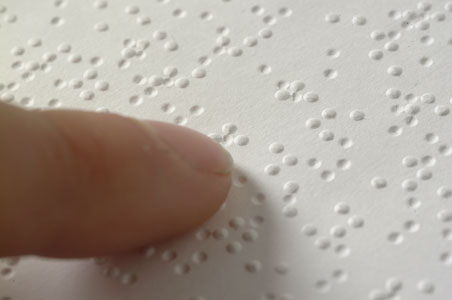
\includegraphics[width=0.2529\linewidth]{braille}
		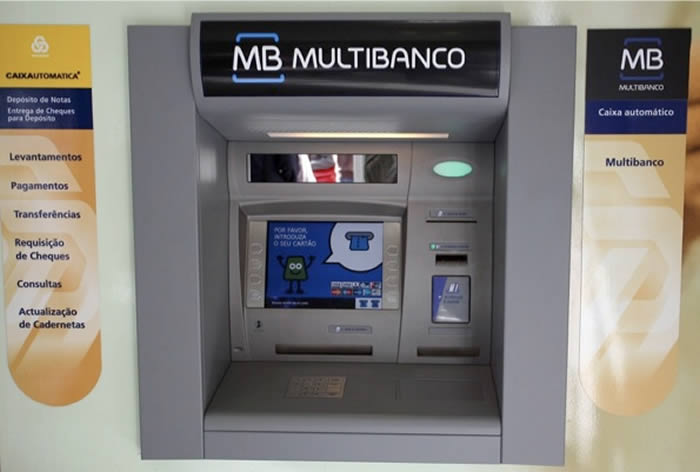
\includegraphics[width=0.2489\linewidth]{atm}
		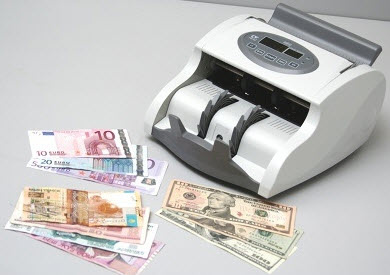
\includegraphics[width=0.2379\linewidth]{counting-machine}
		\captionof{figure}{Examples of applications of banknote recognition systems}
	\end{tikzfigure}


	\section*{Objectives}
	Implementation of a generic banknote recognition system capable of recognizing banknotes with:
	\begin{multicols}{2}
		\begin{itemize}
			\item Partial occlusions
			\item Folding
			\item Wrinkles
			\item Worn / damaged paper
			\item Multiple perspective views
			\item Multiple scales
			\item Environment clutter
			\item Variable lighting conditions
			\item Several banknotes in same image
		\end{itemize}
	\end{multicols}
}

	\block{Recognition System}{
	\section*{Overview}
	Fig. 2 presents the main processing stages of the implemented banknote recognition system. The C++ source code along with the complete results are available at \url{https://github.com/carlosmccosta/Currency-Recognition}.

	\centering
	\begin{minipage}[t]{.66\linewidth}
		\begin{tikzfigure}
			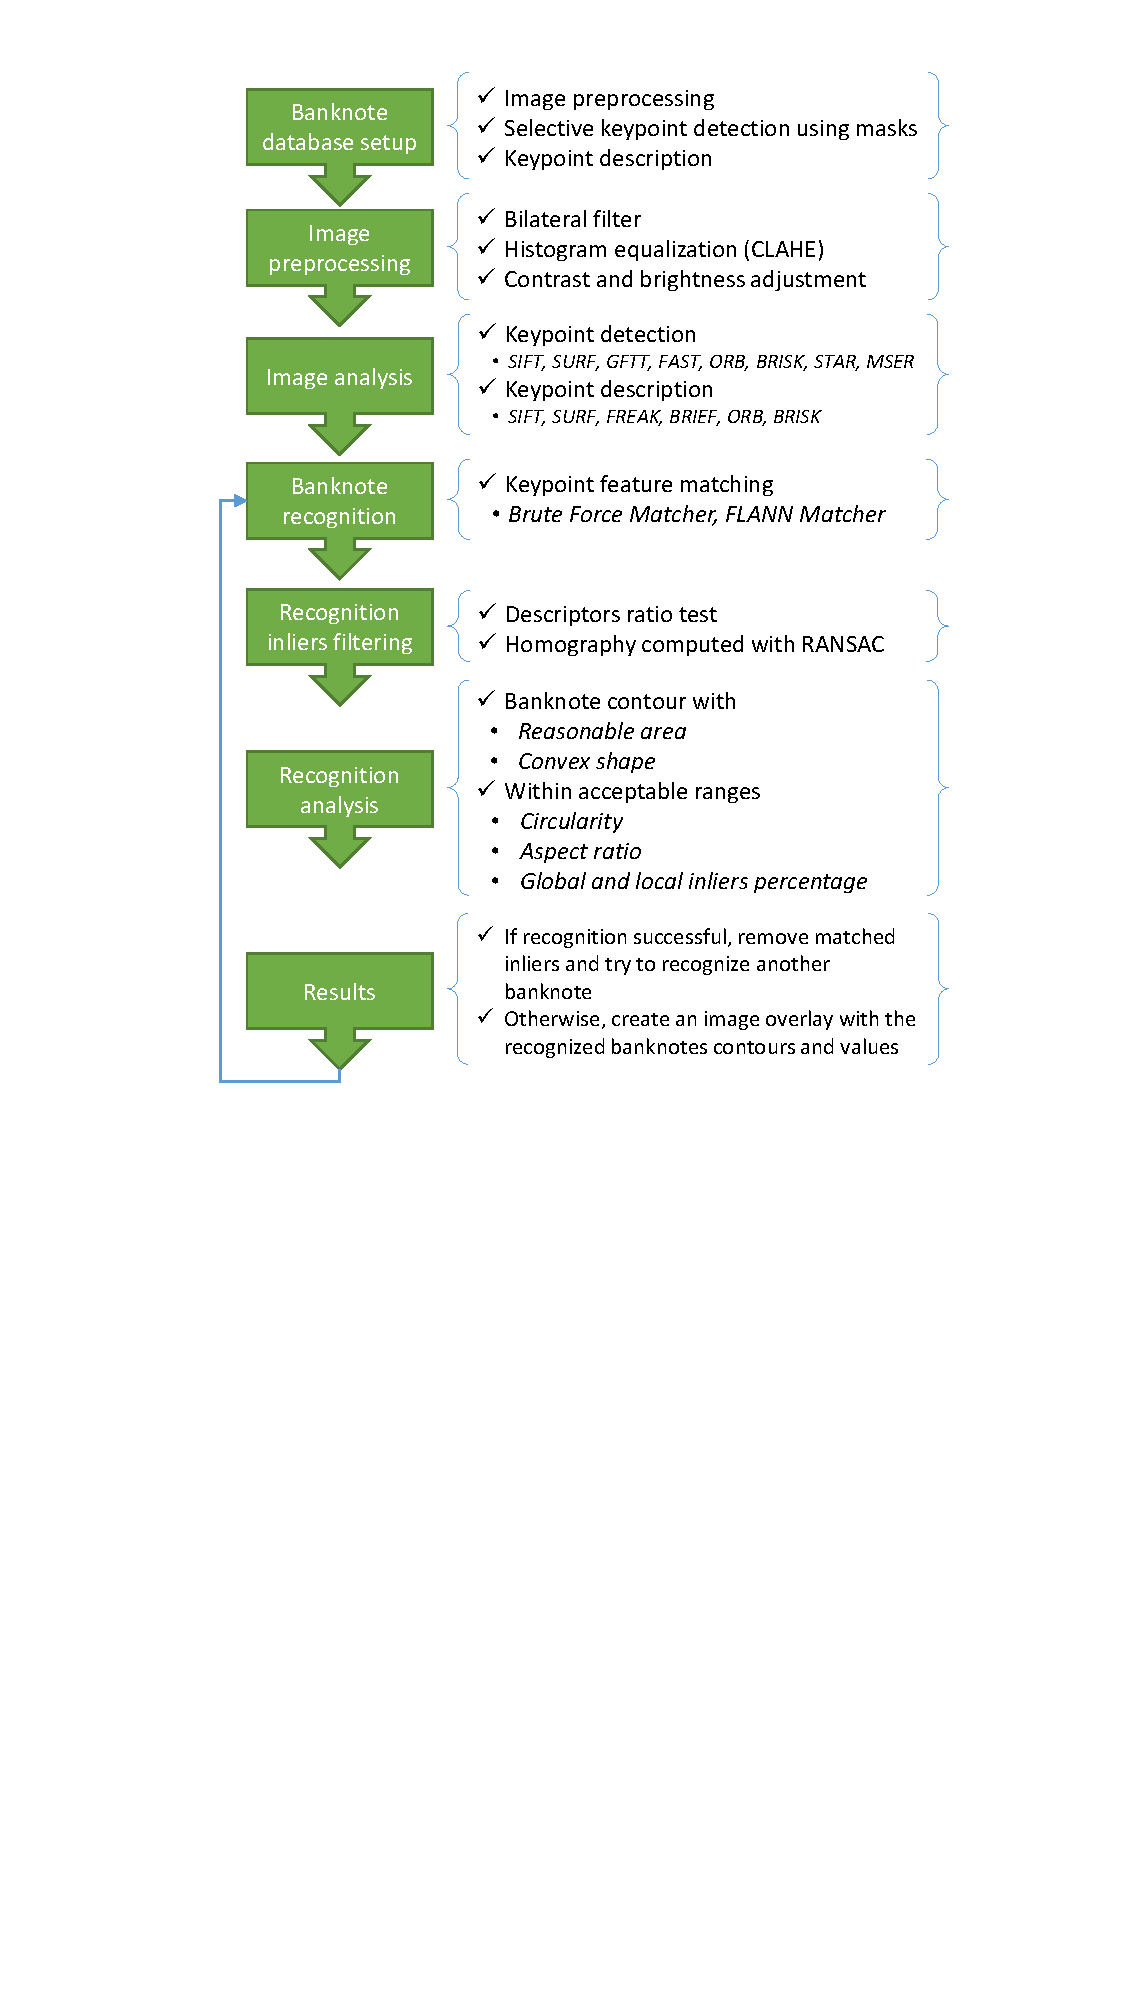
\includegraphics[width=\linewidth]{system-overview}
			\captionof{figure}{Overview of main processing modules}
		\end{tikzfigure}
	\end{minipage}
	\begin{minipage}[t]{.33\linewidth}
		\begin{tikzfigure}
			\centering

			\vspace*{.37em}
			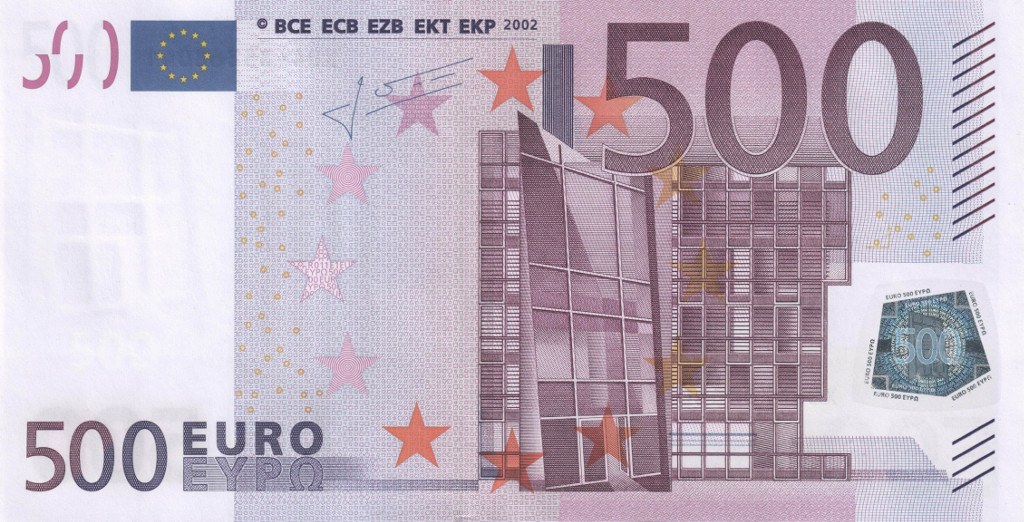
\includegraphics[width=.485\linewidth]{notes-masks/500eu-front}
			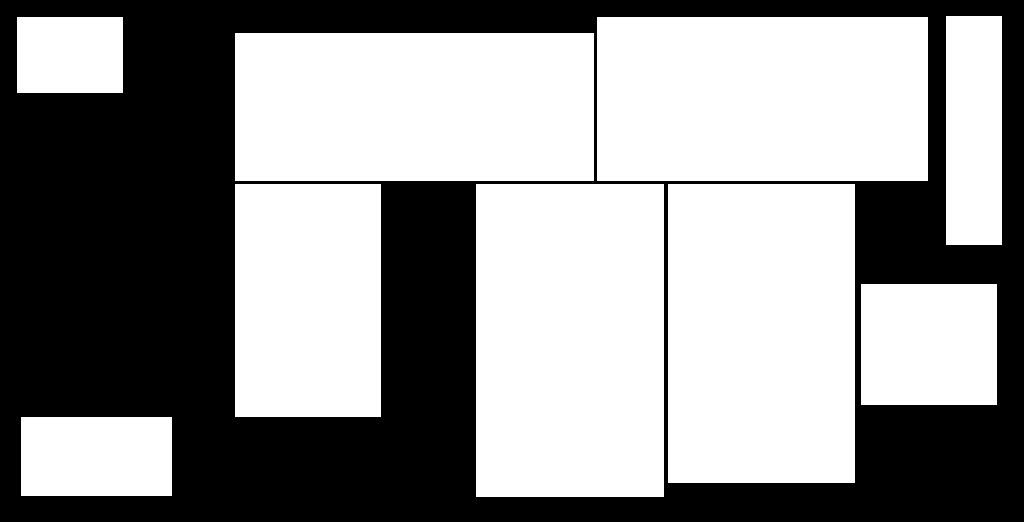
\includegraphics[width=.485\linewidth]{notes-masks/500eu-front-mask}

			\vspace*{0.8em}
			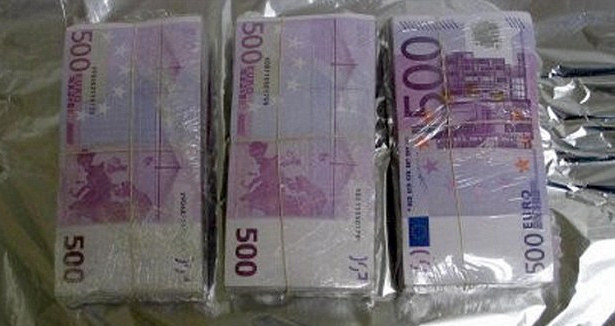
\includegraphics[width=.485\textwidth]{preprocessing/500-500-500}
			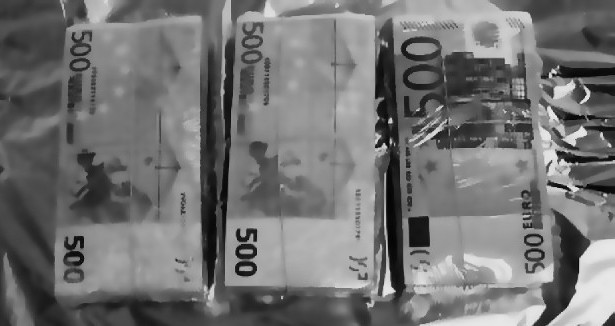
\includegraphics[width=.485\textwidth]{preprocessing/500-500-500-preprocessed}

			\vspace*{1.2em}
			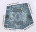
\includegraphics[width=.2496\textwidth]{image-resolution/500eu-front-very-low}\hfill
			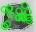
\includegraphics[width=.2496\textwidth]{image-resolution/500eu_front_currencyDB_veryLowResolution_SIFT-Detector}\hfill
			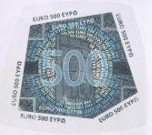
\includegraphics[width=.2499\textwidth]{image-resolution/500eu-front-medium}\hfill
			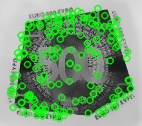
\includegraphics[width=.2499\textwidth]{image-resolution/500eu_front_currencyDB_mediumResolution_SIFT-Detector}

			\vspace*{.9em}
			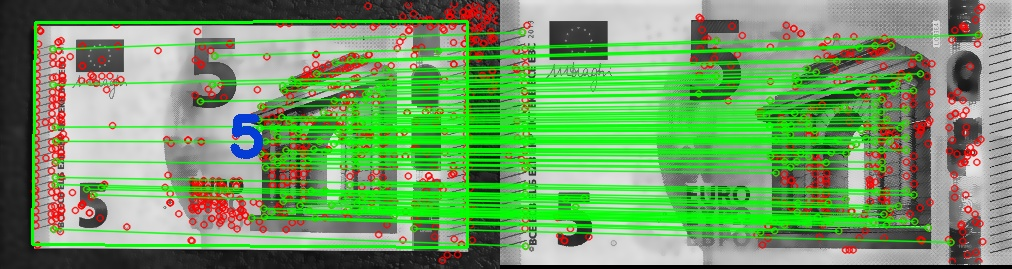
\includegraphics[width=.99\textwidth]{notes-recognition/5__(5).jpg___SIFT-Detector_SIFT-Extractor_BF-Matcher_lowQualityImageDB_globalMatch__inliersMatches__0}
			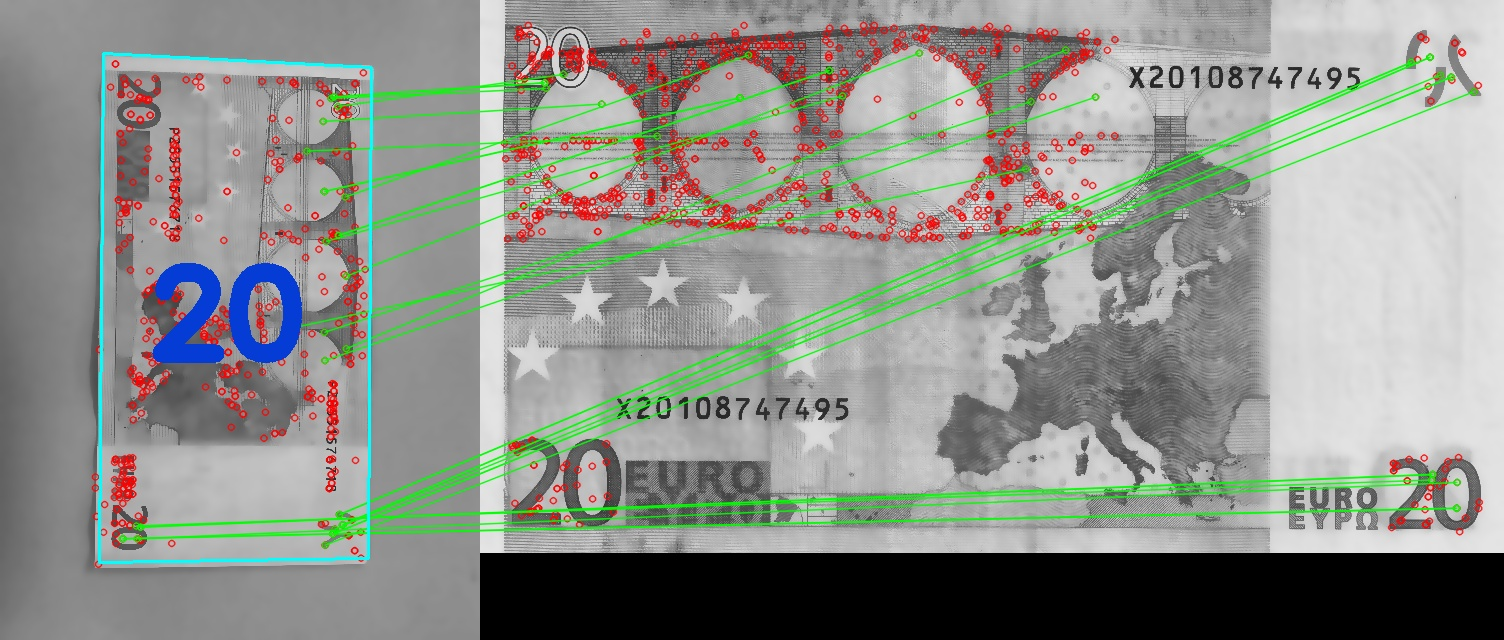
\includegraphics[width=.8\textwidth]{notes-recognition/20__(13).jpg___SIFT-Detector_SIFT-Extractor_BF-Matcher_mediumQualityImageDB_globalMatch__inliersMatches__0}

			\vspace*{.8em}
			
\includegraphics[width=0.75\textwidth]{notes-masks/currency-db-shapes}

			\vspace*{.5em}
			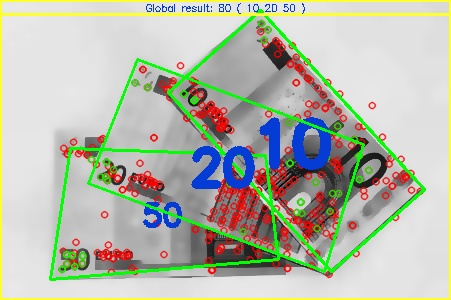
\includegraphics[width=0.8\textwidth]{notes-recognition/10-20-50.jpg___SIFT-Detector_SIFT-Extractor_BF-Matcher_dynamicQualityImageDB_globalMatch}
		\end{tikzfigure}
	\end{minipage}
}

	
	\column{0.5}
	\block{Results}{
	\section*{Results Overview}
	The recognition system successfully detected all the banknotes in the 80 test images (67 images with 1 banknote, 11 images with 2 banknotes and 2 images with 3 banknotes).
	\begin{tikzfigure}
		\centering
		\small
		\tabulinesep = 0.3ex
		\begin{tabu} to \linewidth { X[4.2,l,m] X[l,m] X[l,m] X[l,m] X[l,m] X[l,m] X[l,m] X[l,m] }
			\textbf{Banknote value} & 5\,\euro{} & 10\,\euro{} & 20\,\euro{} & 50\,\euro{} & 100\,\euro{} & 200\,\euro{} & 500\,\euro{}	\\
			\noalign{\vskip 1mm}
			\hline
			\noalign{\vskip 1mm}
			\textbf{Nº of banknotes}			& 15		 & 12		   & 19			 & 19		   & 6			  & 9			 & 15			\\
		\end{tabu}
		\captionof{table}{Testing dataset overview}
	\end{tikzfigure}


	\begin{tikzfigure}
		\centering
		\small
		\tabulinesep = 0.3ex
		\begin{tabu} to \linewidth { X[0.6,c,m] X[0.8,c,m] X[c,m] X[c,m] X[c,m] }
			\rowfont{\bfseries\itshape} Detector & Descriptor & Images with 1 banknote & Images with 2 banknotes & Images with 3 banknotes \\
			\noalign{\vskip 2mm} 
			\hline
			\noalign{\vskip 2mm} 
			SIFT	 & SIFT		  & 37			   & 7				  & 2	\\
			SURF	 & SURF		  & 24			   & 3				  & 0	\\
			GFTT	 & SIFT		  & 3			   & 1				  & 0	\\
			FAST	 & SIFT		  & 1			   & 0				  & 0	\\
			BRISK	 & BRISK	  & 1			   & 0				  & 0	\\
			ORB		 & ORB		  & 1			   & 0				  & 0	\\
		\end{tabu}
		\captionof{table}{Selection of the configurations with the best recognition results (1 configuration per test image)}
	\end{tikzfigure}


	\section*{Banknote Recognition}
	Figures 3 to 10 show some representative recognition test results.

	\begin{minipage}[b]{.47\linewidth}
		\begin{tikzfigure}
			\centering
			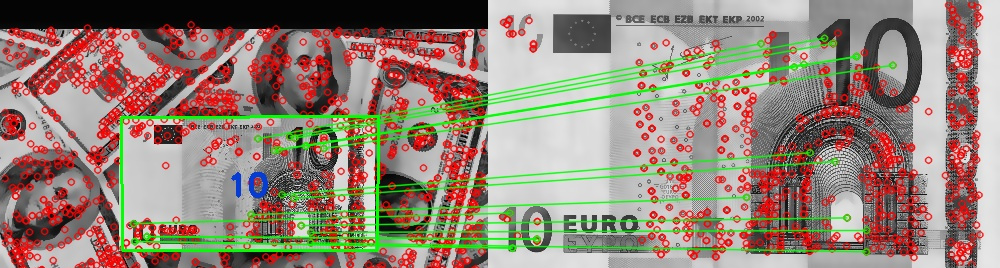
\includegraphics[width=\linewidth]{notes-recognition/10__(9).jpeg___SIFT-Detector_SIFT-Extractor_BF-Matcher_lowQualityImageDB_globalMatch__inliersMatches__0}
			\captionof{figure}{Detection of a banknote in an ideal perspective view with background clutter (using SIFT detector, SIFT descriptors and BFMatcher)}
		\end{tikzfigure}
	\end{minipage}
	\begin{minipage}[b]{.47\linewidth}
		\begin{tikzfigure}
			\centering
			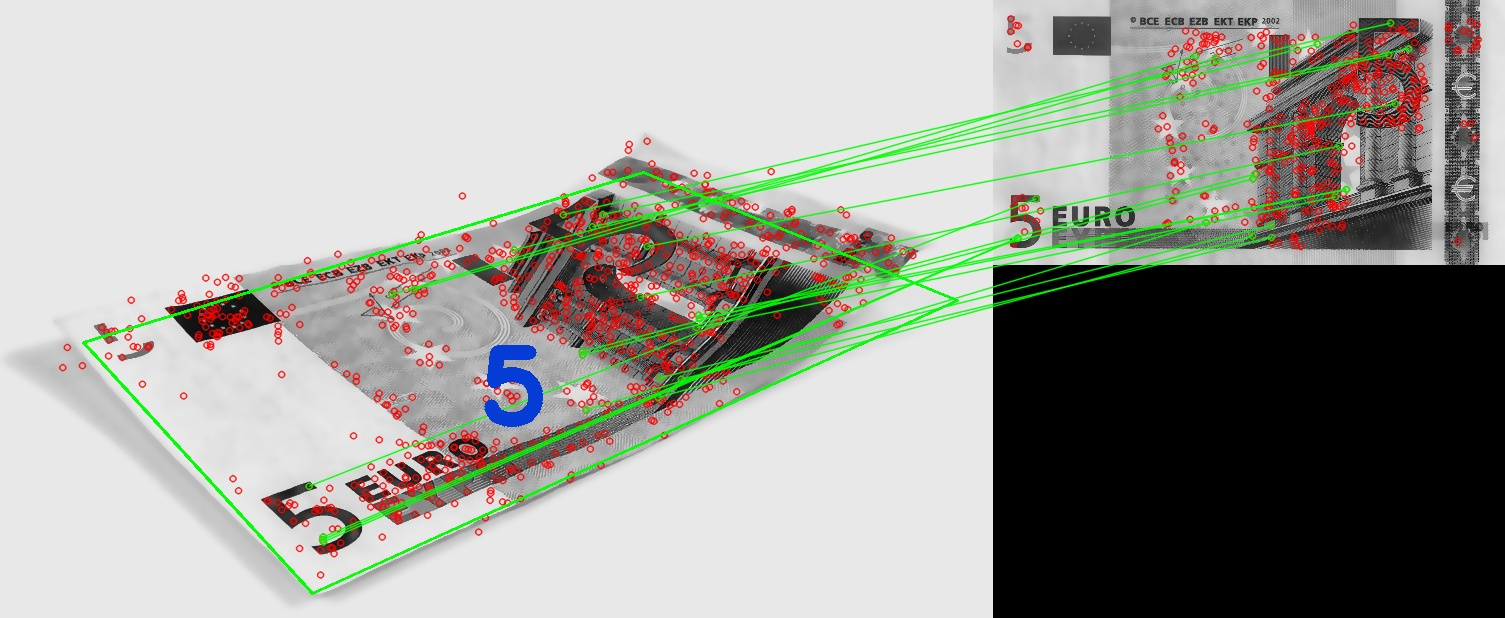
\includegraphics[width=\linewidth]{notes-recognition/5__(6).jpg___SURF-Detector_SURF-Extractor_BF-Matcher_lowQualityImageDB_globalMatch__inliersMatches__0}
			\captionof{figure}{Detection of a banknote with perspective distortion and folding (using SURF detector, SURF descriptors and BFMatcher)}
		\end{tikzfigure}
	\end{minipage}


	\begin{minipage}[b]{.47\linewidth}
		\begin{tikzfigure}
			\centering
			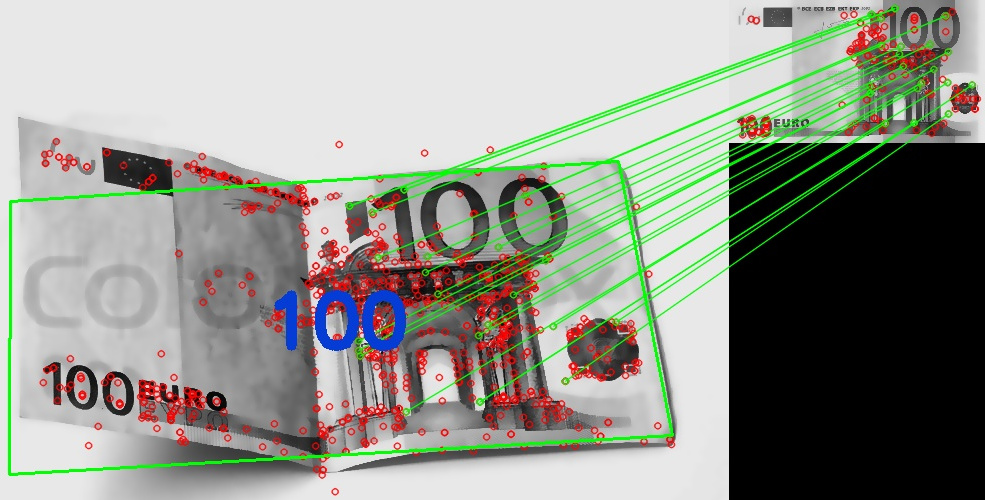
\includegraphics[width=\linewidth]{notes-recognition/100__(4).jpg___SIFT-Detector_SIFT-Extractor_BF-Matcher_dynamicQualityImageDB_globalMatch__inliersMatches__0.jpg}
			\captionof{figure}{Detection of a partially folded banknote\\(using SIFT detector, SIFT descriptors and BFMatcher)}
		\end{tikzfigure}
	\end{minipage}
	\begin{minipage}[b]{.47\linewidth}
		\begin{tikzfigure}
			\centering
			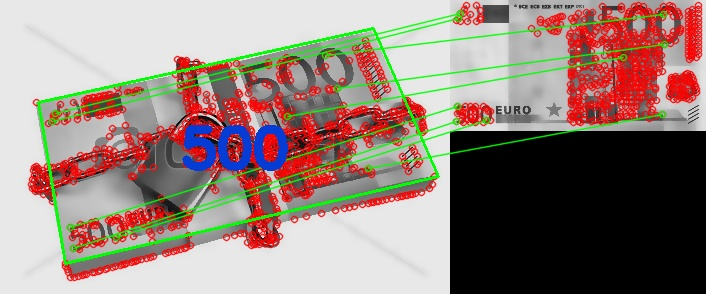
\includegraphics[width=\linewidth]{notes-recognition/500.jpg___GFTT-Detector_SIFT-Extractor_BF-Matcher_dynamicQualityImageDB_globalMatch__inliersMatches__0}
			\captionof{figure}{Detection of a partially occluded banknote\\(using GFTT detector, SIFT descriptors and BFMatcher)}
		\end{tikzfigure}
	\end{minipage}


	\begin{minipage}[b]{.47\linewidth}
		\begin{tikzfigure}
			\centering
			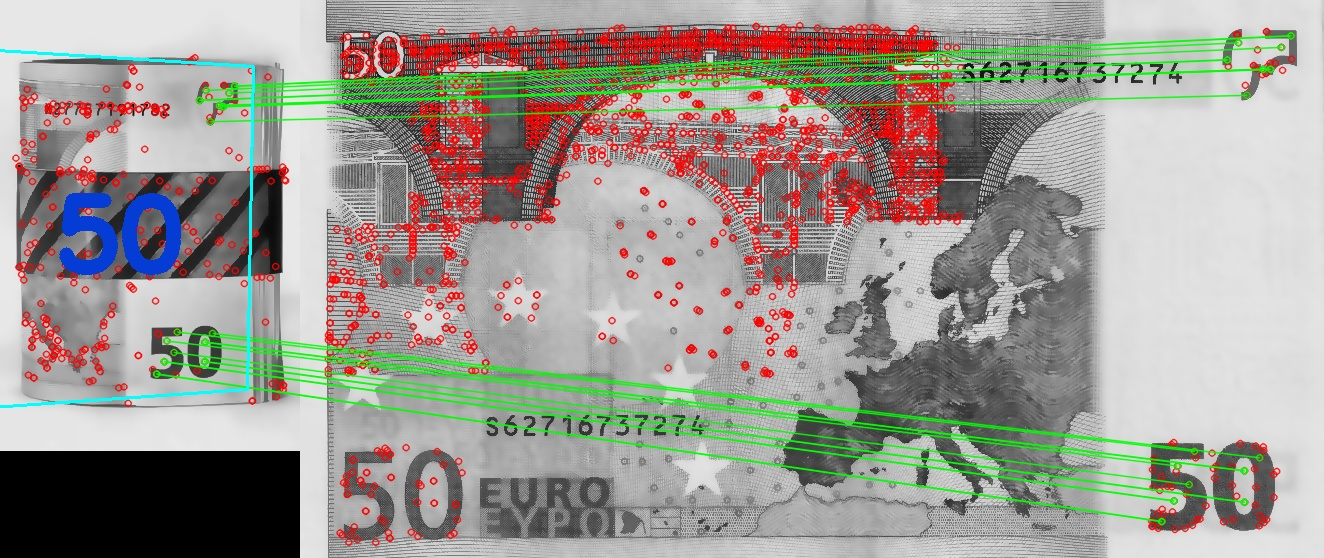
\includegraphics[width=\linewidth]{notes-recognition/50__(13).jpg___SIFT-Detector_SIFT-Extractor_BF-Matcher_mediumQualityImageDB_globalMatch__inliersMatches__0}
			\captionof{figure}{Detection of a partially visible banknote\\(using SIFT detector, SIFT descriptors and BFMatcher)}
		\end{tikzfigure}
	\end{minipage}
	\begin{minipage}[b]{.47\linewidth}
		\begin{tikzfigure}
			\centering
			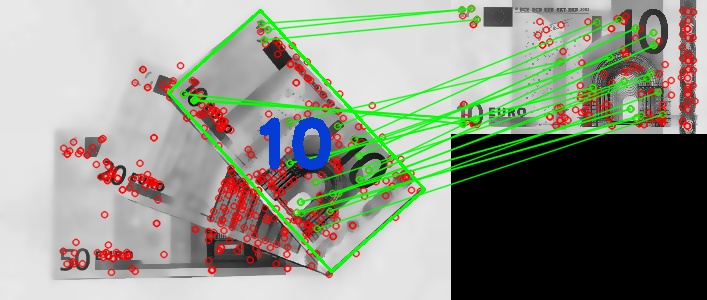
\includegraphics[width=\linewidth]{notes-recognition/10-20-50.jpg___SIFT-Detector_SIFT-Extractor_BF-Matcher_dynamicQualityImageDB_globalMatch__inliersMatches__1}
			\captionof{figure}{Detection of the first overlapping banknote\\(using SIFT detector, SIFT descriptors and BFMatcher)}
		\end{tikzfigure}
	\end{minipage}


	\begin{minipage}[b]{.47\linewidth}
		\begin{tikzfigure}
			\centering
			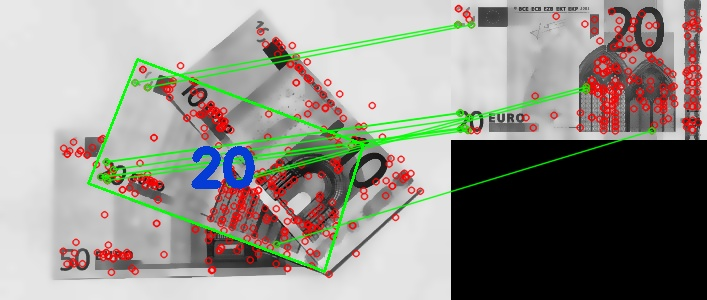
\includegraphics[width=\linewidth]{notes-recognition/10-20-50.jpg___SIFT-Detector_SIFT-Extractor_BF-Matcher_dynamicQualityImageDB_globalMatch__inliersMatches__2}
			\captionof{figure}{Detection of the second overlapping banknote\\(using SIFT detector, SIFT descriptors and BFMatcher)}
		\end{tikzfigure}
	\end{minipage}
	\begin{minipage}[b]{.47\linewidth}
		\begin{tikzfigure}
			\centering
			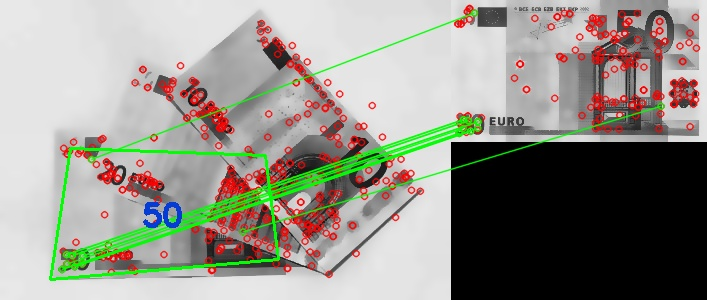
\includegraphics[width=\linewidth]{notes-recognition/10-20-50.jpg___SIFT-Detector_SIFT-Extractor_BF-Matcher_dynamicQualityImageDB_globalMatch__inliersMatches__0}
			\captionof{figure}{Detection of the third overlapping banknote\\(using SIFT detector, SIFT descriptors and BFMatcher)}
		\end{tikzfigure}
	\end{minipage}
}

	\block{Summary}{
	\begin{itemize}
		\item The proposed recognition system managed to detect all the 95 Euro banknotes in the 80 test images
		\item It was robust enough to handle folded and wrinkled banknotes with different kinds of illumination and perspective views
		\item The system is extensible to other banknote currencies and can also be used to detect planar objects besides banknotes
	\end{itemize}
}

\end{columns}

\end{document}
\endinput
